\documentclass{article}

\usepackage{tikz}
\usepackage{tikz-dimline}
\usetikzlibrary{shapes,arrows,shadows}
\usepackage{amsmath,bm,times}
\begin{document}
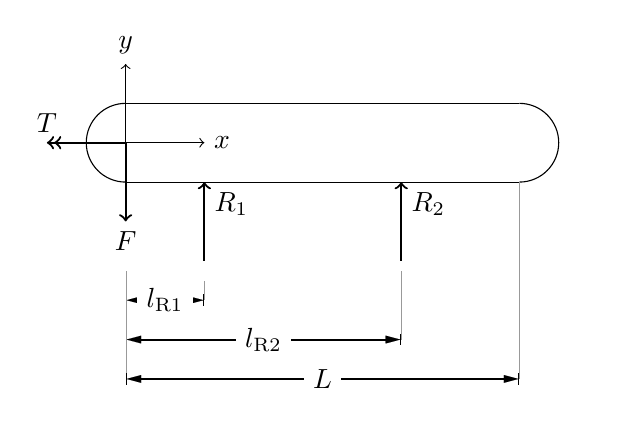
\begin{tikzpicture}[scale=0.5]




\begin{scope}
\clip [rotate=0] (-2,2) rectangle (0,-2);
\draw (0,0) circle [radius=1cm];
\end{scope}

\coordinate (O) at (0,0) ;
% Second cirle middle point
\coordinate (A) at (3.5,-6.06217); 
\coordinate (B) at (3.5+6.06217,-6.06217-3.5);
\coordinate (L1) at (10,0);

	% Lenght of pendulums are 7cm

	% Axis for underactuated Pendulum
	\draw[->] (0,0) -- (2,0) node[anchor=west] {$x$};
	\draw[->] (0,0) -- (0,2) node[anchor=south] {$y$};
	\draw[dashed] (0,0) -- (0,-2);
	
	%%%%%%%%%%%%%%%%%%%%%%%%%%%%%%%%%%%%%%%%%%%%%%%%%%%%%%%%%%%%%%%%%%%%%%%%%%%%%%

	%%%%%%%%%%%%%%%%%%%%%%%%%%%%%%%%%%%%%%%%%%%%%%%%%%%%%%%%%%%%%%%%%%%%%%%%%%%%%%
	
	%%%%%%%%%%%%%%%%%%%%%%%%%%%%%%%%%%%%%%%%%%%%%%%%%%%%%%%%%%%%%%%%%%%%%%%%%%%%%%
				%% Middle line for underactuated pendulum %%
	%\draw[dashed] (O) -- ([yshift=-4cm]L2);
	%%%%%%%%%%%%%%%%%%%%%%%%%%%%%%%%%%%%%%%%%%%%%%%%%%%%%%%%%%%%%%%%%%%%%%%%%%%%%%
	
		
	%%%%%%%%%%%%%%%%%%%%%%%%%%%%%%%%%%%%%%%%%%%%%%%%%%%%%%%%%%%%%%%%%%%%%%%%%%%%%%

	%%%%%%%%%%%%%%%%%%%%%%%%%%%%%%%%%%%%%%%%%%%%%%%%%%%%%%%%%%%%%%%%%%%%%%%%%%%%%%

	%Long lines for Beam
	\draw[] (0,1) -- ([yshift=1cm]L1);
	\draw[] (0,-1) -- 	([yshift=-1cm]L1);	
	
	%%%%%%%%%%%%%%%%%%%%%%%%%%%%%%%%%%%%%%%%%%%%%%%%%%%%%%%%%%%%%%%%%%%%%%%%%%%%%%
	%% Circle at the right %%
	
	\begin{scope}
	\clip [rotate=0] ([yshift=-2cm]L1) rectangle ([xshift=2cm,yshift=2cm]L1);
	\draw (L1) circle [radius=1cm];
	\end{scope}
	
	%% Reaction Forces
	\draw[->,thick] ([xshift=-8cm,yshift=-3cm]L1) -- ([xshift=-8cm,yshift=-1cm]L1) node[below right]{$R_{1}$};
	\draw[->,thick] ([xshift=-3cm,yshift=-3cm]L1) -- ([xshift=-3cm,yshift=-1cm]L1) node[below right]{$R_{2}$};
	
	%% Applied Forces
	\draw[->,thick] (0,0) -- (0,-2) node[below]{$F$};
	\draw[->>,thick] (0,0) -- (-2,0)node[above]{$T$};
	
						%% Dimensions of Beam %%
	\dimline[line style = {line width=0.7},extension start length=-0.25, extension end length=-0.25]{(0,-4)}{(2,-4)}{$l_{\text{R1}}$}
	
	\dimline[line style = {line width=0.7},extension start length=-0.25, extension end length=-0.25]{(0,-5)}{(7,-5)}{$l_{\text{R2}}$}
	
	\dimline[line style = {line width=0.7},extension start length=-0.25, extension end length=-0.5]{(0,-6)}{(10,-6)}{$L$}
	




	
\end{tikzpicture}
\end{document}